\appendix 
\refstepcounter{chapter}
%
% Usability-Test
%
%\section{Usability-Test} 
\label{app:Usability}
\subsection{Ablauf, Beschreibung, Evaluationsbogen}
% ------------------------------
% Bild Usability Beschreibung
% ------------------------------
\begin{figure}[H]
	\centering
		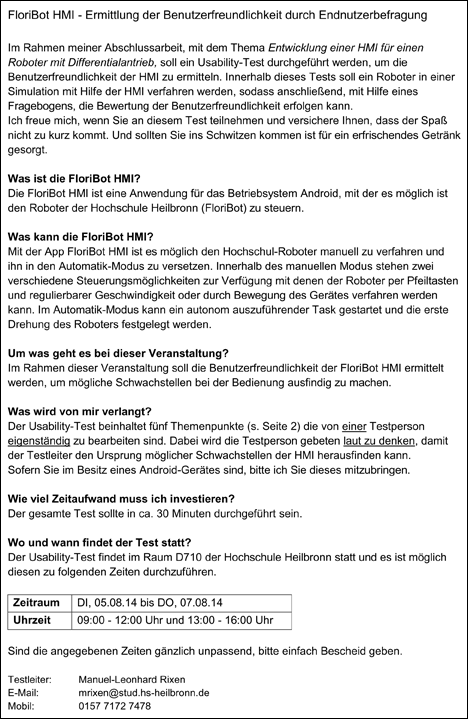
\includegraphics[width=0.85\textwidth]{03_Grafiken/Anhang/UsabilityBogen/UsabilityBeschreibung.png}
	\caption[Beschreibung des Usability-Tests]{Beschreibung des Usability-Tests}
	\label{fig:UsabilityBeschreibung}
\end{figure}
% ------------------------------
% Bild Usability Ablauf
% ------------------------------
\begin{figure}[H]
	\centering
		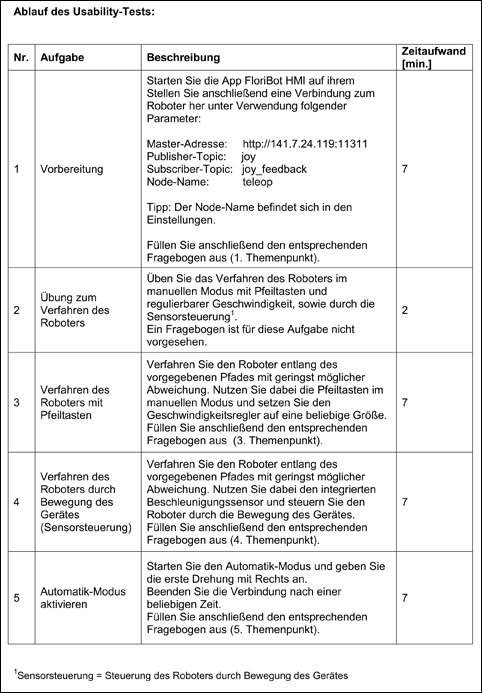
\includegraphics[width=0.85\textwidth]{03_Grafiken/Anhang/UsabilityBogen/UsabilityAblauf.png}
	\caption[Ablauf des Usability-Tests]{Ablauf des Usability-Tests}
	\label{fig:UsabilityAblauf}
\end{figure}
% ------------------------------
% Bilder des Usability Evaluationsbogens
% ------------------------------
\begin{figure}[H]
	\centering
		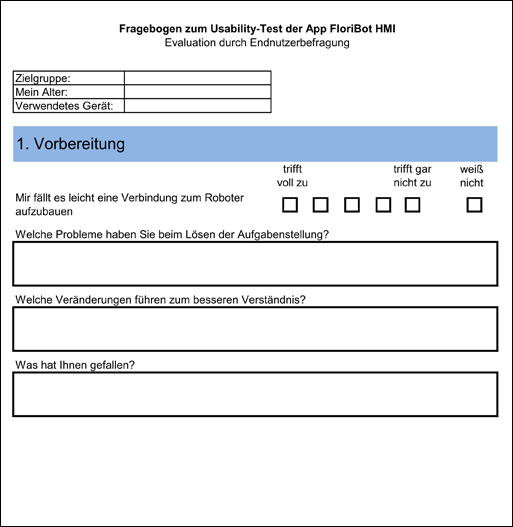
\includegraphics[width=0.85\textwidth]{03_Grafiken/Anhang/UsabilityBogen/UsabilityEvaluationsbogen.png}
	\caption[Evaluationsbogen des Usability-Tests - Seite 1]{Evaluationsbogen des Usability-Tests - Seite 1}
	\label{fig:UsabilityEvaluationsbogen}
\end{figure}
\newpage
\begin{figure}[H]
	\centering
		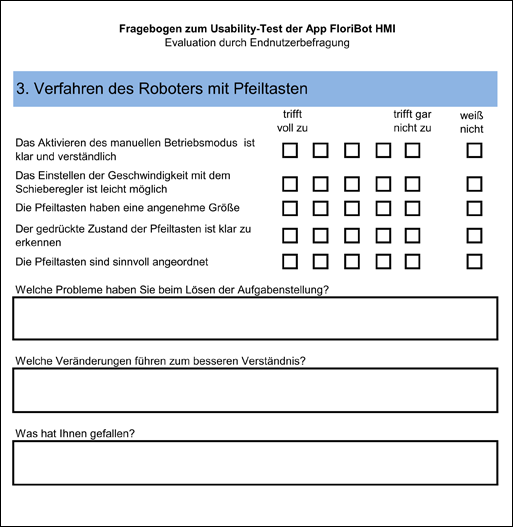
\includegraphics[width=0.85\textwidth]{03_Grafiken/Anhang/UsabilityBogen/UsabilityEvaluationsbogen1.png}
	\caption[Evaluationsbogen des Usability-Tests - Seite 2]{Evaluationsbogen des Usability-Tests - Seite 2}
	\label{fig:UsabilityEvaluationsbogen}
\end{figure}
\newpage
\begin{figure}[H]
	\centering
		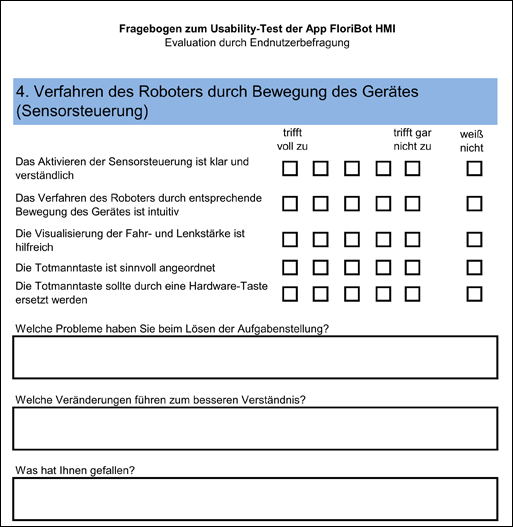
\includegraphics[width=0.85\textwidth]{03_Grafiken/Anhang/UsabilityBogen/UsabilityEvaluationsbogen2.png}
	\caption[Evaluationsbogen des Usability-Tests - Seite 3]{Evaluationsbogen des Usability-Tests - Seite 3}
	\label{fig:UsabilityEvaluationsbogen}
\end{figure}
\newpage
\begin{figure}[H]
	\centering
		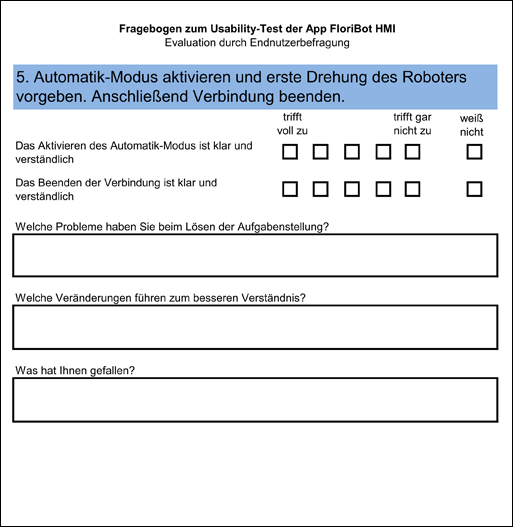
\includegraphics[width=0.85\textwidth]{03_Grafiken/Anhang/UsabilityBogen/UsabilityEvaluationsbogen3.png}
	\caption[Evaluationsbogen des Usability-Tests - Seite 4]{Evaluationsbogen des Usability-Tests - Seite 4}
	\label{fig:UsabilityEvaluationsbogen}
\end{figure}
\newpage
\begin{figure}[H]
	\centering
		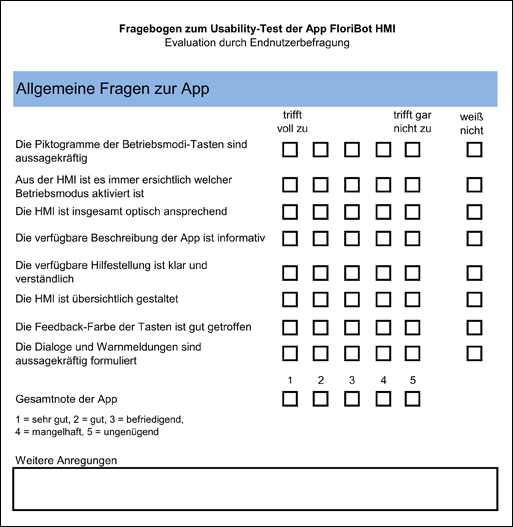
\includegraphics[width=0.85\textwidth]{03_Grafiken/Anhang/UsabilityBogen/UsabilityEvaluationsbogen4.png}
	\caption[Evaluationsbogen des Usability-Tests - Seite 5]{Evaluationsbogen des Usability-Tests - Seite 5}
	\label{fig:UsabilityEvaluationsbogen}
\end{figure}
\newpage
\newpage
\subsection{Diagramme}
\label{app:UsabilityKreisdiagramme}
% ------------------------------
% Aufgabenteil 3 - Aussage 1
% ------------------------------
\begin{figure}[H]
	\centering
		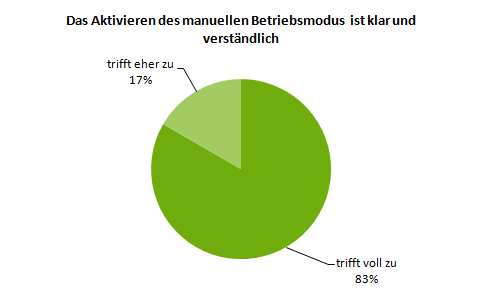
\includegraphics[width=0.85\textwidth]{03_Grafiken/Anhang/UsabilityDiagramme/Aufgabenteil3Aussage1.png}
	\caption[Diagramm zum Analysieren der Benutzerfreundlichkeit beim Verfahren mit Pfeiltasten - Aussage 1]{Diagramm zum Analysieren der Benutzerfreundlichkeit beim Verfahren mit Pfeiltasten - Aussage 1}
	\label{fig:Aufgabenteil3Aussage1}
\end{figure}
% ------------------------------
% Aufgabenteil 3 - Aussage 2
% ------------------------------
\begin{figure}[H]
	\centering
		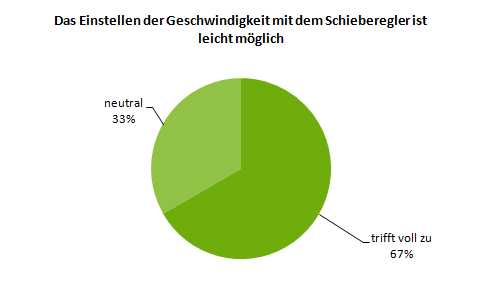
\includegraphics[width=0.85\textwidth]{03_Grafiken/Anhang/UsabilityDiagramme/Aufgabenteil3Aussage2.png}
	\caption[Diagramm zum Analysieren der Benutzerfreundlichkeit beim Verfahren mit Pfeiltasten - Aussage 2]{Diagramm zum Analysieren der Benutzerfreundlichkeit beim Verfahren mit Pfeiltasten - Aussage 2}
	\label{fig:Aufgabenteil3Aussage2}
\end{figure}
% ------------------------------
% Aufgabenteil 3 - Aussage 3
% ------------------------------
\begin{figure}[H]
	\centering
		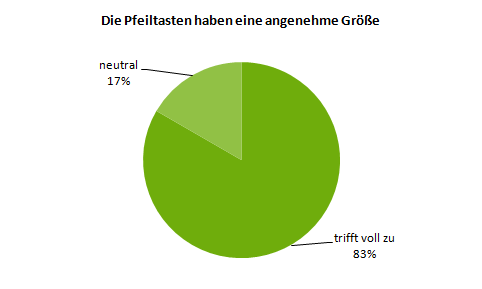
\includegraphics[width=0.85\textwidth]{03_Grafiken/Anhang/UsabilityDiagramme/Aufgabenteil3Aussage3.png}
	\caption[Diagramm zum Analysieren der Benutzerfreundlichkeit beim Verfahren mit Pfeiltasten - Aussage 3]{Diagramm zum Analysieren der Benutzerfreundlichkeit beim Verfahren mit Pfeiltasten - Aussage 3}
	\label{fig:Aufgabenteil3Aussage3}
\end{figure}
% ------------------------------
% Aufgabenteil 3 - Aussage 4
% ------------------------------
\begin{figure}[H]
	\centering
		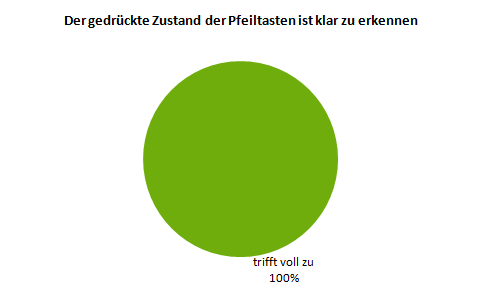
\includegraphics[width=0.85\textwidth]{03_Grafiken/Anhang/UsabilityDiagramme/Aufgabenteil3Aussage4.png}
	\caption[Diagramm zum Analysieren der Benutzerfreundlichkeit beim Verfahren mit Pfeiltasten - Aussage 4]{Diagramm zum Analysieren der Benutzerfreundlichkeit beim Verfahren mit Pfeiltasten - Aussage 4}
	\label{fig:Aufgabenteil3Aussage4}
\end{figure}
% ------------------------------
% Aufgabenteil 3 - Aussage 5
% ------------------------------
\begin{figure}[H]
	\centering
		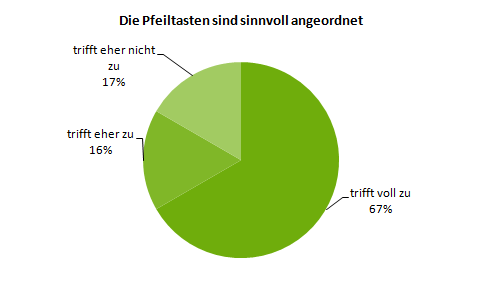
\includegraphics[width=0.85\textwidth]{03_Grafiken/Anhang/UsabilityDiagramme/Aufgabenteil3Aussage5.png}
	\caption[Diagramm zum Analysieren der Benutzerfreundlichkeit beim Verfahren mit Pfeiltasten - Aussage 5]{Diagramm zum Analysieren der Benutzerfreundlichkeit beim Verfahren mit Pfeiltasten - Aussage 5}
	\label{fig:Aufgabenteil3Aussage5}
\end{figure}
% ------------------------------
% Aufgabenteil 4 - Aussage 1
% ------------------------------
\begin{figure}[H]
	\centering
		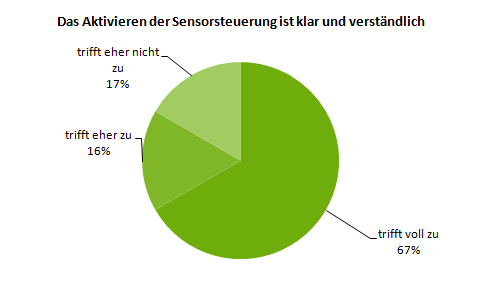
\includegraphics[width=0.85\textwidth]{03_Grafiken/Anhang/UsabilityDiagramme/Aufgabenteil4Aussage1.png}
	\caption[Diagramm zum Analysieren der Benutzerfreundlichkeit bei der Sensorsteuerung - Aussage 1]{Diagramm zum Analysieren der Benutzerfreundlichkeit bei der Sensorsteuerung - Aussage 1}
	\label{fig:Aufgabenteil4Aussage1}
\end{figure}
% ------------------------------
% Aufgabenteil 4 - Aussage 2
% ------------------------------
\begin{figure}[H]
	\centering
		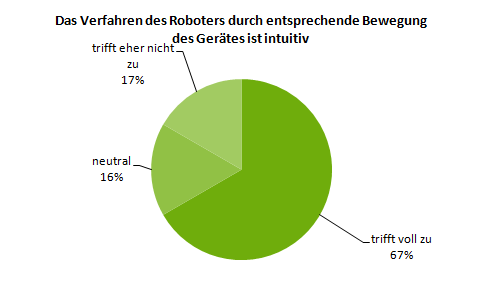
\includegraphics[width=0.85\textwidth]{03_Grafiken/Anhang/UsabilityDiagramme/Aufgabenteil4Aussage2.png}
	\caption[Diagramm zum Analysieren der Benutzerfreundlichkeit bei der Sensorsteuerung - Aussage 1]{Diagramm zum Analysieren der Benutzerfreundlichkeit bei der Sensorsteuerung - Aussage 2}
	\label{fig:Aufgabenteil4Aussage2}
\end{figure}
% ------------------------------
% Aufgabenteil 4 - Aussage 2
% ------------------------------
\begin{figure}[H]
	\centering
		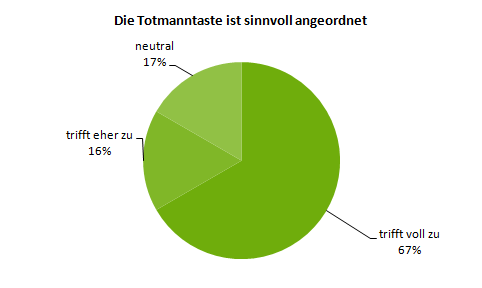
\includegraphics[width=0.85\textwidth]{03_Grafiken/Anhang/UsabilityDiagramme/Aufgabenteil4Aussage4.png}
	\caption[Diagramm zum Analysieren der Benutzerfreundlichkeit bei der Sensorsteuerung - Aussage 4]{Diagramm zum Analysieren der Benutzerfreundlichkeit bei der Sensorsteuerung - Aussage 4}
	\label{fig:Aufgabenteil4Aussage4}
\end{figure}
% ------------------------------
% Aufgabenteil 5 - Aussage 2
% ------------------------------
\begin{figure}[H]
	\centering
		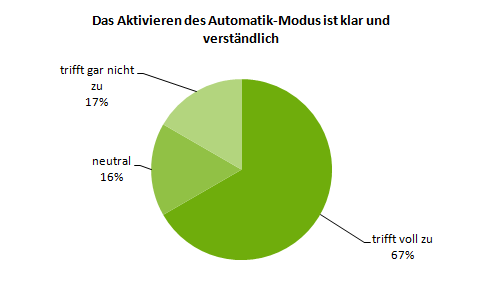
\includegraphics[width=0.85\textwidth]{03_Grafiken/Anhang/UsabilityDiagramme/Aufgabenteil5Aussage1.png}
	\caption[Diagramm zum Analysieren der Benutzerfreundlichkeit im Automatik-Modus - Aussage 1]{Diagramm zum Analysieren der Benutzerfreundlichkeit im Automatik-Modus - Aussage 1}
	\label{fig:Aufgabenteil5Aussage1}
\end{figure}
% ------------------------------
% Aufgabenteil 5 - Aussage 2
% ------------------------------
\begin{figure}[H]
	\centering
		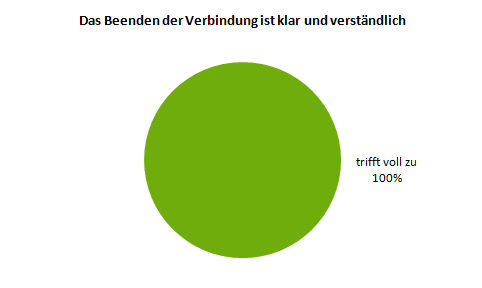
\includegraphics[width=0.85\textwidth]{03_Grafiken/Anhang/UsabilityDiagramme/Aufgabenteil5Aussage2.png}
	\caption[Diagramm zum Analysieren der Benutzerfreundlichkeit im Automatik-Modus - Aussage 2]{Diagramm zum Analysieren der Benutzerfreundlichkeit im Automatik-Modus - Aussage 2}
	\label{fig:Aufgabenteil5Aussage2}
\end{figure}
%
% Klassendiagramme
%
\newpage
%\section{Klassendiagramme}
\label{app:Klassendiagramme}
\subsection{Name Klasse 1}
%
% Bild der Klasse NAME
%
\begin{figure}[H]
\centering

\includegraphics[width=0.7\linewidth]{03_Grafiken/Anhang/Klassendiagramme/pseudoImage}
\caption[Klasse NAME]{Klasse NAME}
\label{fig:pseudoimage}
\end{figure}


%
% Details der Klasse NAME
%
\begin{center}
\renewcommand{\arraystretch}{1.2} 
\newcolumntype{C}[1]{>{\centering\arraybackslash}p{#1}}
\centering
\begin{longtable}{|p{2cm}p{12cm}|}
\caption{Parameter der Klasse NAME}\label{tab:KlasseParameter-NAME}\\
\hline 
\multicolumn{2}{|l|}{\cellcolor{gray}\textbf{Attribute}} \\ 
\hline 
\multicolumn{2}{|l|}{Element-Name + Datentyp (z.B. Button)}\\
 & Beschreibung der Funktion \\ 
\hline 
\multicolumn{2}{|l|}{Element-Name + Datentyp (z.B. Button)} \\
\multicolumn{2}{|l|}{Weitere Element-Namen + Datentyp (z.B. Button)} \\
& Beschreibung der Funktion \\ 
\hline 
%
% METHODEN
%
\multicolumn{2}{|l|}{\cellcolor{gray}\textbf{Methoden}} \\ 
\hline 
\multicolumn{2}{|l|}{Funktion-Name (z.B. protected void NAME())} \\ 
& Beschreibung der Funktion  \\
\hline 
\multicolumn{2}{|l|}{Funktion-Name (z.B. protected void NAME())} \\
& Beschreibung der Funktion \\ 
\hline 
%
% SCHNITTSTELLEN
%
\multicolumn{2}{|l|}{\cellcolor{gray}\textbf{Schnittstellen}} \\ 
\hline 
\multicolumn{2}{|l|}{Schnittstellen-Name (z.B. public interface NAME())} \\ 
\multicolumn{2}{|l|}{Funktion-Name (z.B. public void NAME())} \\ 
& Beschreibung der Schnittstelle  \\
\hline 
\end{longtable} 
\end{center}
\newpage
\subsection{Name Klasse 2}
%
% Bild der Klasse NAME
%
\begin{figure}[H]
	\centering
	
\includegraphics[width=0.7\linewidth]{03_Grafiken/pseudoImage}
	\caption[Klasse NAME]{Klasse NAME}
	\label{fig:pseudoimage}
\end{figure}

%
% Details der Klasse NAME
%
\begin{center}
	\renewcommand{\arraystretch}{1.2} 
	\newcolumntype{C}[1]{>{\centering\arraybackslash}p{#1}}
	\centering
	\begin{longtable}{|p{2cm}p{12cm}|}
		\caption{Parameter der Klasse NAME}\label{tab:KlasseParameter-NAME}\\
		\hline 
		\multicolumn{2}{|l|}{\cellcolor{gray}\textbf{Attribute}} \\ 
		\hline 
		\multicolumn{2}{|l|}{Element-Name + Datentyp (z.B. Button)}\\
		& Beschreibung der Funktion \\ 
		\hline 
		\multicolumn{2}{|l|}{Element-Name + Datentyp (z.B. Button)} \\
		\multicolumn{2}{|l|}{Weitere Element-Namen + Datentyp (z.B. Button)} \\
		& Beschreibung der Funktion \\ 
		\hline 
		%
		% METHODEN
		%
		\multicolumn{2}{|l|}{\cellcolor{gray}\textbf{Methoden}} \\ 
		\hline 
		\multicolumn{2}{|l|}{Funktion-Name (z.B. protected void NAME())} \\ 
		& Beschreibung der Funktion  \\
		\hline 
		\multicolumn{2}{|l|}{Funktion-Name (z.B. protected void NAME())} \\
		& Beschreibung der Funktion \\ 
		\hline 
		%
		% SCHNITTSTELLEN
		%
		\multicolumn{2}{|l|}{\cellcolor{gray}\textbf{Schnittstellen}} \\ 
		\hline 
		\multicolumn{2}{|l|}{Schnittstellen-Name (z.B. public interface NAME())} \\ 
		\multicolumn{2}{|l|}{Funktion-Name (z.B. public void NAME())} \\ 
		& Beschreibung der Schnittstelle  \\
		\hline 
	\end{longtable} 
\end{center}
%
% Ablauf der Anwendungsfalldiagramme
%
%\section{Ablauf der Anwendungsfalldiagramme}
\label{app:UseCasesAblauf}
\begin{table}[H]
\caption{Ablauf: NAME}\label{app:UseCaseNAME2}
\renewcommand{\arraystretch}{1.5} 
\newcolumntype{C}[1]{>{\centering\arraybackslash}p{#1}}
\centering
\begin{tabular}{|p{1.5cm}|p{1.5cm}|p{9cm}|}
 	\hline 
    \multicolumn{2}{|l|}{\cellcolor{hellgrau}\textbf{Name}} & Manuelles Verfahren des Roboters \\     
    \hline
    \multicolumn{2}{|l|}{\cellcolor{hellgrau}\textbf{Ziel}} & Verfahren des Roboters mit Tasten \\
    \hline
    \multicolumn{2}{|l|}{\cellcolor{hellgrau}\textbf{Akteure}} & Bediener, Roboter \\   
    \hline
    \multicolumn{2}{|l|}{\cellcolor{hellgrau}\textbf{Trigger}} & Starten des Steuerungsmen�s durch Bet�tigen der Verbindungstaste  \\   
    \hline
    \multicolumn{2}{|l|}{\cellcolor{hellgrau}\textbf{Vorbedingung}} & Aktive Datenverbindung zum Roboter \\   
    \specialrule{2pt}{0pt}{0pt} 
    \rowcolor{hellgrau} \textbf{Schritt} & \textbf{Akteur} & \textbf{Ablauf} \\
    \hline
    1. & Person & Aktivieren des manuellen Betriebsmodus \\
    \hline
    2. & Person & Einstellen der gew�nschten Geschwindigkeit \\
    \hline
    3. & Person & Verfahren des Roboters in die gew�nschte Ausgangsorientierung \\
    \hline
    4. & Roboter & Abarbeiten der empfangenen Beschleunigungswerte \\
    \hline
\end{tabular} 
\end{table}
\begin{table}[H]
\caption{Ablauf: NAME}\label{app:UseCaseNAME1}
\renewcommand{\arraystretch}{1.5} 
\newcolumntype{C}[1]{>{\centering\arraybackslash}p{#1}}
\centering
\begin{tabular}{|p{1.5cm}|p{1.5cm}|p{9cm}|}
 	\hline 
    \multicolumn{2}{|l|}{\cellcolor{hellgrau}\textbf{Name}} & Verbindung einrichten \\     
    \hline
    \multicolumn{2}{|l|}{\cellcolor{hellgrau}\textbf{Ziel}} & Verbindung zum Roboter aufbauen \\
    \hline
    \multicolumn{2}{|l|}{\cellcolor{hellgrau}\textbf{Akteure}} & Bediener \\   
    \hline
    \multicolumn{2}{|l|}{\cellcolor{hellgrau}\textbf{Trigger}} & Starten der Anwendung FloriBot HMI \\   
    \hline
    \multicolumn{2}{|l|}{\cellcolor{hellgrau}\textbf{Vorbedingung}} & Flugmodus ist aktiv \\   
    \specialrule{2pt}{0pt}{0pt} 
    \rowcolor{hellgrau} \textbf{Schritt} & \textbf{Akteur} & \textbf{Ablauf} \\
    \hline
    1. & Person & Eingabe der Master-Adresse \\
    \hline
    2. & Person & Eingabe des Publisher-Topics \\
    \hline
    3. & Person & Eingabe des Subscriber-Topics \\
    \hline
    4. & Person & Eingabe des Node Namens im Optionsmen� \\
    \hline
    5. & Person & Setzen des Themes im Optionsmen� \\
    \hline
    6. & Person & Bet�tigen der Verbindungstaste zum Starten des Verbindungsaufbaus \\
	\hline 
	\rowcolor{hellgrau} & & \textbf{Erweiterung} \\
	7.a &  & Kein Verbindungsaufbau m�glich, wenn Flugmodus deaktiviert. Ein Hinweis wird ausgegeben. \\
    \hline
    7.b &  & Kein Verbindungsaufbau m�glich, wenn nicht alle Eingabefelder ausgef�llt sind. Ein Hinweis wird ausgegeben. \\
    \hline
    7.c &  & Kein Verbindungsaufbau m�glich, wenn Wlan-Schnittstelle deaktiviert ist. Ein Hinweis wird ausgegeben. \\
	\hline 
\end{tabular} 
\end{table}
%
% Listings
%
\section{Listings}
\label{app:Quellcode}
\subsection{Listing 1}
\label{app:Listing1}
\begin{lstlisting}[language=Java, caption=NAME]
public void Function {

}
\end{lstlisting}
%
% --------------------------------------------
%
\begin{lstlisting}[language=Java, caption=NAME]
public void Function {

}
\end{lstlisting}
\newpage
\subsection{Listing 2}
\label{app:Listing2}
\begin{lstlisting}[language=Java, caption=NAME]
public void Function {

}
\end{lstlisting}
%
% --------------------------------------------
%
\begin{lstlisting}[language=Java, caption=NAME]
public void Function {

}
\end{lstlisting}
%
% Fehlermeldungen und Bugs
%
%\section{Fehlermeldungen und Bugs}
\label{FehlerBugs}
In der folgend dargestellten Tabelle sind die derzeit vorhandenen Bugs der Software \textit{NAME} aufgelistet. Dabei wird, neben einer Beschreibung des Fehlers, der Kontext genannt, in dem das Auftreten erfolgt und ein Indikator aufgezeigt, der die Bedeutung des Fehlers wiedergibt.\\
Die Farben des Indikators sind definiert mit:
\begin{table}[H]
\centering
\begin{tabular}{ll}
\textcolor{red}{Rot:} & Stark \\ 
\textcolor{yellow}{Gelb:} & Mittel \\ 
\textcolor{green}{Gr�n:} & Schwach \\ 
\end{tabular} 
\end{table}

\begin{table}[H]
\caption{Liste von bekannten Bugs der Software NAME HMI}\label{app:BugListe}
\renewcommand{\arraystretch}{1.5} 
\newcolumntype{C}[1]{>{\centering\arraybackslash}p{#1}}
\centering
\begin{tabular}{|p{4.5cm}|p{3cm}|C{6cm}|}
 	\hline 
    \rowcolor{hellgrau} \textbf{Fehlerbeschreibung} & \textbf{Kontext} & \textbf{Sicherheitsbeeintr�chtigung}\\
    \hline
    Fehlerbeschreibung & Kontext & \redDot{-0.4} \\
    \hline
    Fehlerbeschreibung & Kontext & \redDot{-1.3} \\
    \hline
    Fehlerbeschreibung & Kontext & \greenDot{-0.6} \\
    \hline
    Fehlerbeschreibung & Kontext & \yellowDot{-1.2} \\
    \hline
    Fehlerbeschreibung & Kontext & \greenDot{-1.2} \\
    \hline
    Fehlerbeschreibung & Kontext & \greenDot{-1.2} \\
    \hline
\end{tabular} 
\end{table}

\newpage
Folgende Tabelle zeigt eine �bersicht der Fehlermeldungen, durch die der Bediener der Software \gls{NAME} �ber m�gliche fehlerhafte Eingaben und nicht unterst�tzte Handhabung informiert wird. Dabei ist, neben der Beschreibung der Fehlermeldung, der Kontext, indem der Fehler auftritt und der L�sungsvorschlag genannt.
\begin{table}[htb]
\caption{Fehlermeldungen der Software NAME}\label{app:Fehlermeldungen}
\renewcommand{\arraystretch}{1.5} 
\newcolumntype{C}[1]{>{\centering\arraybackslash}p{#1}}
\centering
\begin{tabular}{|p{4.5cm}|p{4.5cm}|p{4.5cm}|}
 	\hline 
    \rowcolor{hellgrau} \textbf{Fehlermeldung} & \textbf{Kontext} & \textbf{L�sung} \\
    \hline
    Fehlermeldung & Kontext & L�sung \\
    \hline
    Fehlermeldung & Kontext & L�sung \\
    \hline
    Fehlermeldung & Kontext & L�sung\\
    \hline
    Fehlermeldung & Kontext & L�sung\\
    \hline
    Fehlermeldung & Kontext & L�sung\\
    \hline
    Fehlermeldung & Kontext & L�sung\\
    \hline
    Fehlermeldung & Kontext & L�sung\\
    \hline
    Fehlermeldung & Kontext & L�sung\\
    \hline
    Fehlermeldung & Kontext & L�sung
\end{tabular} 
\end{table}
%
% Erklaerung
%
\postappendix
\listoffigures
\listoftables
\printglossary[type=\acronymtype]%, style=listdotted
\printglossary
%\addchap{Verzeichnis Daten-CD}
%Dieses Verzeichnis zeigt die wichtigsten Bestandteile der Daten-CD. Dabei stellt das Zeichen + einen Ordner und das Zeichen - eine Datei dar.

\vspace{1cm}
\parbox{0cm}{\begin{tabbing}
x \= x \= x \= x \= x \= x \kill
- Datei1 \\
- Datei2 \\
+ Ordner1 \\
+ Ordner2 \\
\> + Unterordner1-Ebene1 \\
\>\> + Unterordner1-Ebene2 \\
\>\>\> + Unterordner1-Ebene3 \\
\>\>\>\> + Unterordner1-Ebene4 \\
\>\>\>\> + Unterordner2-Ebene4 \\
\>\>\>\> + ... \\
\>\> + Unterordner2-Ebene2 \\
\>\>\> - Datei \\
\>\> + Unterordner3-Ebene2 \\
\>\>\> + Unterordner2-Ebene3 \\
\>\>\> + Unterordner3-Ebene3 \\
\>\>\> + ... \\
+ Ordner3 \\
\> + Unterordner2-Ebene1 \\
\>\> + Unterordner4-Ebene2 \\
\>\>\> + Unterordner1-Ebene4 \\
\end{tabbing}}
\addchap{Erkl�rung} 
\refstepcounter{chapter}
%\section{Erkl�rung}
Hiermit erkl�re ich an Eides Statt, dass ich die vorliegende Arbeit selbst�ndig und ohne 
Benutzung anderer als der angegebenen Hilfsmittel angefertigt habe. Die aus fremden 
Quellen direkt oder indirekt �bernommenen Gedanken sind als solche kenntlich gemacht. 

ORT, {DATUM}
%\\[30pt]
\vspace{-0.2cm}
\begin{figure}[H]
	
\includegraphics[width=0.25\textwidth]{03_Grafiken/Anhang/mySignature.jpg}
\end{figure}
\vspace{-1cm}
Manuel-Leonhard Rixen

%%\section{Verwendete Symbole und Begriffe}
%%\input{99_Anhang/SymboleBegriffe}	